\documentclass[11pt,a4paper]{article}

\usepackage{fontspec}
\IfFontExistsTF{Times New Roman}{\setmainfont{Times New Roman}}{%
  \IfFontExistsTF{Arial}{\setmainfont{Arial}}{\setmainfont{TeX Gyre Termes}}%
}
\usepackage{amsmath,amssymb}
\usepackage{geometry}
\geometry{top=1.4cm,bottom=1.4cm,left=1.6cm,right=1.6cm}
\usepackage{xcolor}
\usepackage{array,booktabs}
\usepackage{float}
\usepackage{enumitem}
\usepackage{fancyhdr}
\usepackage{tikz}
\usetikzlibrary{arrows.meta,calc,positioning}
\usepackage{hyperref}
\hypersetup{colorlinks=true,linkcolor=blue!50!black,urlcolor=blue!50!black}

\setlength{\parindent}{0pt}
\setlength{\parskip}{2.6pt}
\setlength{\abovecaptionskip}{4pt}
\setlength{\belowcaptionskip}{1pt}
\setlength{\textfloatsep}{8pt}
\setlength{\floatsep}{6pt}
\setlength{\intextsep}{6pt}
\renewcommand{\arraystretch}{1.15}
\renewcommand{\figurename}{Hình}
\renewcommand{\tablename}{Bảng}

\definecolor{criticalbar}{RGB}{211,47,47}
\definecolor{normalbar}{RGB}{63,125,190}
\definecolor{weekend}{RGB}{232,232,232}

\pagestyle{fancy}
\fancyhf{}
\lhead{\small Quản trị dự án -- Bài 01 PERT}
\rhead{\small Bach Minh Quang -- 202490077}
\cfoot{\thepage}
\setlength{\headheight}{13pt}

\tikzset{
  event/.style={circle,draw=black,thick,minimum size=11mm,inner sep=0.5pt,
    font=\scriptsize\bfseries,align=center,fill=white},
  arc/.style={-{Latex[length=2.1mm]},thick,normalbar},
  criticalarc/.style={-{Latex[length=2.1mm]},very thick,criticalbar},
  dummyarc/.style={-{Latex[length=2.1mm]},dashed,thick,gray!60!black},
  arclabel/.style={font=\scriptsize\bfseries,fill=white,inner sep=1pt}
}

\newcommand{\ganttrowseven}[5]{%
  \node[anchor=east,font=\scriptsize] at (-0.22,-#1+0.16) {#2};%
  \pgfmathtruncatemacro{\gLast}{#4-1}%
  \foreach \gK in {0,...,\gLast}{%
    \pgfmathtruncatemacro{\gStart}{#3+\gK}%
    \fill[#5] (\gStart,-#1) rectangle ++(1,0.32);%
  }%
}
\newcommand{\ganttrowfive}[5]{%
  \node[anchor=east,font=\scriptsize] at (-0.22,-#1+0.16) {#2};%
  \pgfmathtruncatemacro{\gLast}{#4-1}%
  \foreach \gK in {0,...,\gLast}{%
    \pgfmathtruncatemacro{\gWork}{#3+\gK}%
    \pgfmathtruncatemacro{\gWeek}{int(\gWork/5)}%
    \pgfmathtruncatemacro{\gCal}{\gWork+2*\gWeek}%
    \fill[#5] (\gCal,-#1) rectangle ++(1,0.32);%
  }%
}

\begin{document}

\begin{center}
  {\large\bfseries ĐẠI HỌC BÁCH KHOA HÀ NỘI}\\[1pt]
  {\bfseries Trường Công nghệ Thông tin và Truyền thông}\\[5pt]
  {\Large\bfseries BÀI 01 -- SƠ ĐỒ PERT, DỰ TRỮ VÀ ĐƯỜNG GĂNG}\\[2pt]
  {\small Bach Minh Quang \quad MSSV: 202490077 \quad Hà Nội, 09/2026}
\end{center}
\vspace{-3pt}
\hrule
\vspace{7pt}

Mạng AOA: đỉnh $=$ sự kiện, cung $=$ công việc. Trong vòng tròn: số hiệu và $t_s/t_m$.
Cung đỏ $=$ găng, xanh $=$ không găng, nét đứt $=$ việc giả ($d=0$).

\vspace{2pt}
\begin{table}[H]\centering
\caption{Dữ liệu công việc}
\small
\begin{tabular}{cccccc}
\toprule
\textbf{CV} & \textbf{Trình tự} & \textbf{$d$} & \textbf{CV} & \textbf{Trình tự} & \textbf{$d$}\\
\midrule
$A$ & Từ đầu & 2 & $G$ & Từ đầu & 3\\
$B$ & Sau $A$ & 1 & $H$ & Sau $D,G$ & 3\\
$C$ & Từ đầu & 1 & $F$ & Từ đầu & 2\\
$D$ & Sau $B,C$ & 1 & $I$ & Sau $H,F$ & 2\\
\bottomrule
\end{tabular}
\end{table}

\paragraph{a. Sơ đồ PERT}
Ba việc giả: $e_1$ nối kết thúc $C$ vào đầu $D$; $e_2$ nối kết thúc $G$ vào đầu $H$; $e_3$ nối kết thúc $F$ vào đầu $I$.

\begin{figure}[H]\centering
\resizebox{0.98\linewidth}{!}{%
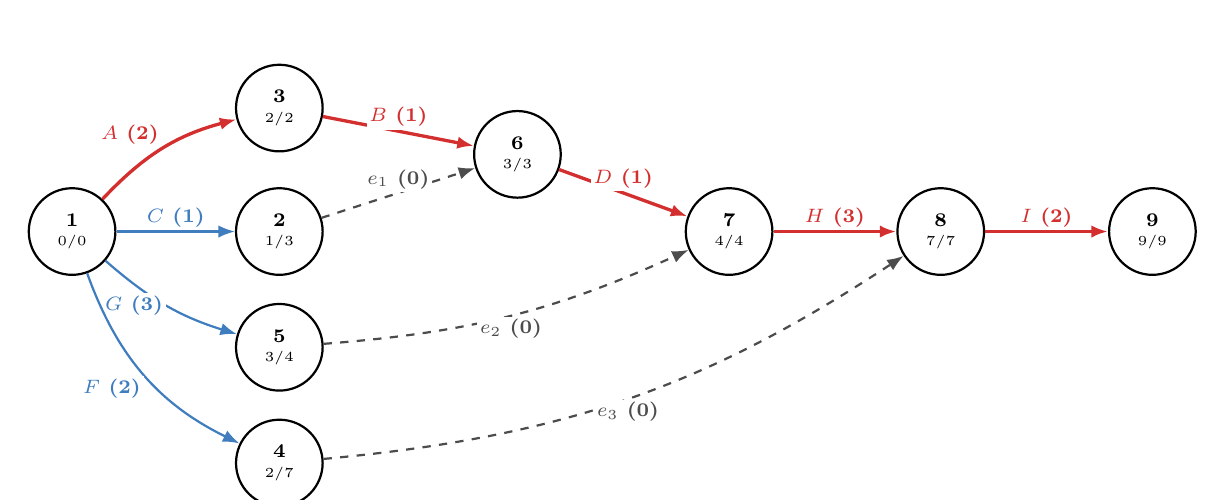
\begin{tikzpicture}[x=1.12cm,y=0.98cm]
  \node[event] (p1) at (0.0,1.55) {1\\[-1pt]{\tiny\normalfont $0/0$}};
  \node[event] (p3) at (2.35,3.15) {3\\[-1pt]{\tiny\normalfont $2/2$}};
  \node[event] (p2) at (2.35,1.55) {2\\[-1pt]{\tiny\normalfont $1/3$}};
  \node[event] (p5) at (2.35,0.05) {5\\[-1pt]{\tiny\normalfont $3/4$}};
  \node[event] (p4) at (2.35,-1.45) {4\\[-1pt]{\tiny\normalfont $2/7$}};
  \node[event] (p6) at (5.05,2.55) {6\\[-1pt]{\tiny\normalfont $3/3$}};
  \node[event] (p7) at (7.45,1.55) {7\\[-1pt]{\tiny\normalfont $4/4$}};
  \node[event] (p8) at (9.85,1.55) {8\\[-1pt]{\tiny\normalfont $7/7$}};
  \node[event] (p9) at (12.25,1.55) {9\\[-1pt]{\tiny\normalfont $9/9$}};

  \draw[criticalarc] (p1) to[bend left=16] node[arclabel,above left] {$A$ (2)} (p3);
  \draw[arc] (p1) -- node[arclabel,above] {$C$ (1)} (p2);
  \draw[arc] (p1) to[bend right=12] node[arclabel,left] {$G$ (3)} (p5);
  \draw[arc] (p1) to[bend right=22] node[arclabel,below left] {$F$ (2)} (p4);
  \draw[criticalarc] (p3) -- node[arclabel,above] {$B$ (1)} (p6);
  \draw[dummyarc] (p2) -- node[arclabel,above] {$e_1$ (0)} (p6);
  \draw[criticalarc] (p6) -- node[arclabel,above] {$D$ (1)} (p7);
  \draw[dummyarc] (p5) to[bend right=10] node[arclabel,below] {$e_2$ (0)} (p7);
  \draw[criticalarc] (p7) -- node[arclabel,above] {$H$ (3)} (p8);
  \draw[dummyarc] (p4) to[bend right=14] node[arclabel,below] {$e_3$ (0)} (p8);
  \draw[criticalarc] (p8) -- node[arclabel,above] {$I$ (2)} (p9);
\end{tikzpicture}}
\caption{Mạng PERT (AOA). Đường găng $A{-}B{-}D{-}H{-}I$.}
\end{figure}

\paragraph{b. Chỉ tiêu sự kiện, thời gian dự án, đường găng}
Tính tiến: $t_s(j)=\max_{i\rightarrow j}\{t_s(i)+d_{ij}\}$, $t_s(1)=0$.
Tính lùi: $t_m(i)=\min_{i\rightarrow j}\{t_m(j)-d_{ij}\}$, $t_m(9)=t_s(9)$.
Dự trữ đỉnh $R(i)=t_m(i)-t_s(i)$; đỉnh găng khi $R=0$.

{\small
\textbf{Tiến:}
$t_s(1)=0$;
$t_s(2)=1$;
$t_s(3)=2$;
$t_s(4)=2$;
$t_s(5)=3$;
$t_s(6)=\max(2+1,\ 1+0)=3$;
$t_s(7)=\max(3+1,\ 3+0)=4$;
$t_s(8)=\max(4+3,\ 2+0)=7$;
$t_s(9)=7+2=9$.
\\
\textbf{Lùi:}
$t_m(9)=9$;
$t_m(8)=7$;
$t_m(7)=4$;
$t_m(6)=3$;
$t_m(5)=4$;
$t_m(4)=7$;
$t_m(3)=2$;
$t_m(2)=3$;
$t_m(1)=\min(0,2,1,5)=0$.
}

\begin{table}[H]\centering
\caption{Thời điểm sớm, muộn và dự trữ sự kiện}
\small
\begin{tabular}{c|ccccccccc}
\toprule
Sự kiện $i$ & 1 & 2 & 3 & 4 & 5 & 6 & 7 & 8 & 9\\
\midrule
$t_s(i)$ & 0 & 1 & 2 & 2 & 3 & 3 & 4 & 7 & 9\\
$t_m(i)$ & 0 & 3 & 2 & 7 & 4 & 3 & 4 & 7 & 9\\
$R(i)$   & 0 & 2 & 0 & 5 & 1 & 0 & 0 & 0 & 0\\
\bottomrule
\end{tabular}
\end{table}

Đỉnh găng: $1,3,6,7,8,9$. Thời gian sớm nhất hoàn thành dự án:
\[
  T = t_s(9) = t_m(9) = \mathbf{9\ \text{ngày}}.
\]
Công việc găng khi $TF_{ij}=t_m(j)-t_s(i)-d_{ij}=0$: $A,B,D,H,I$.
Kiểm tra đường dài nhất: $A{+}B{+}D{+}H{+}I=2{+}1{+}1{+}3{+}2=9$;
$C{+}D{+}H{+}I=7$; $G{+}H{+}I=8$; $F{+}I=4$.
\[
  \boxed{A-B-D-H-I \quad (9\ \text{ngày})}
\]

\paragraph{c. Dự trữ độc lập và kéo dài đồng thời}
Với cung $i\rightarrow j$:
\[
  TF=t_m(j)-t_s(i)-d,\quad
  FF=t_s(j)-t_s(i)-d,\quad
  IF=\max\{0,\ t_s(j)-t_m(i)-d\}.
\]

\begin{table}[H]\centering
\caption{Chỉ tiêu thời gian công việc}
\small
\begin{tabular}{c|c|cc|cc|ccc}
\toprule
CV & $d$ & ES & EF & LS & LF & TF & FF & IF\\
\midrule
$A$ & 2 & 0 & 2 & 0 & 2 & 0 & 0 & 0\\
$B$ & 1 & 2 & 3 & 2 & 3 & 0 & 0 & 0\\
$C$ & 1 & 0 & 1 & 2 & 3 & 2 & 0 & 0\\
$D$ & 1 & 3 & 4 & 3 & 4 & 0 & 0 & 0\\
$G$ & 3 & 0 & 3 & 1 & 4 & 1 & 0 & 0\\
$H$ & 3 & 4 & 7 & 4 & 7 & 0 & 0 & 0\\
$F$ & 2 & 0 & 2 & 5 & 7 & 5 & 0 & 0\\
$I$ & 2 & 7 & 9 & 7 & 9 & 0 & 0 & 0\\
\bottomrule
\end{tabular}
\end{table}

Công việc không găng: $C$ ($TF{=}2$), $G$ ($TF{=}1$), $F$ ($TF{=}5$).
Dự trữ độc lập $IF(C)=IF(G)=IF(F)=0$: không việc nào kéo dài được nếu sự kiện đầu xảy ra muộn nhất và sự kiện cuối xảy ra sớm nhất.

Kéo dài \emph{đồng thời} mọi việc không găng thêm $x$ ngày:
$C{-}D{-}H{-}I$: $7+x\le 9\Rightarrow x\le 2$;
$G{-}H{-}I$: $8+x\le 9\Rightarrow x\le 1$;
$F{-}I$: $4+x\le 9\Rightarrow x\le 5$.
Với $x=1$, $\max(EF_B,EF_C)=\max(3,2)=3$ và $\max(EF_D,EF_G)=\max(4,4)=4$, $H$ và $I$ không trễ. Vậy mức kéo dài đồng thời lớn nhất là \textbf{1 ngày} ($\min TF$ của các việc không găng).

\paragraph{d. Biểu đồ Gantt (tương đương MS Project, in A4)}
MS Project: Auto Scheduled; Predecessor $B{\leftarrow}A$, $D{\leftarrow}B,C$, $H{\leftarrow}D,G$, $I{\leftarrow}H,F$;
bật \textit{Format $\to$ Critical Tasks}.
Lịch 7 ngày: Change Working Time (T7--CN làm việc).
Lịch 5 ngày: Standard (T2--T6). Mốc 0 $=$ thứ Hai; lịch chỉ đổi số ngày lịch.

\begin{figure}[H]\centering
\vspace{-4pt}
\begin{tikzpicture}[x=1.50cm,y=0.34cm]
  \draw[gray!22] (0,0) grid (9,-8);
  \foreach \x in {0,...,9} \node[font=\tiny,anchor=south] at (\x,0.05) {\x};
  \ganttrowseven{0}{A}{0}{2}{criticalbar}
  \ganttrowseven{1}{B}{2}{1}{criticalbar}
  \ganttrowseven{2}{C}{0}{1}{normalbar}
  \ganttrowseven{3}{D}{3}{1}{criticalbar}
  \ganttrowseven{4}{G}{0}{3}{normalbar}
  \ganttrowseven{5}{H}{4}{3}{criticalbar}
  \ganttrowseven{6}{F}{0}{2}{normalbar}
  \ganttrowseven{7}{I}{7}{2}{criticalbar}
  \fill[criticalbar] (0,-8.55) rectangle +(0.45,0.26);
  \node[anchor=west,font=\tiny] at (0.55,-8.42) {Găng};
  \fill[normalbar] (2.2,-8.55) rectangle +(0.45,0.26);
  \node[anchor=west,font=\tiny] at (2.75,-8.42) {Không găng. Kết thúc ngày 9.};
\end{tikzpicture}
\caption{Gantt -- tuần làm việc 7 ngày (trục $=$ ngày lịch).}
\end{figure}

\begin{figure}[H]\centering
\vspace{-6pt}
\begin{tikzpicture}[x=1.08cm,y=0.34cm]
  \foreach \w in {0,1} {\fill[weekend] ({7*\w+5},0) rectangle ({7*\w+7},-8);}
  \draw[gray!22] (0,0) grid (13,-8);
  \foreach \x in {0,...,13} \node[font=\tiny,anchor=south] at (\x,0.05) {\x};
  \ganttrowfive{0}{A}{0}{2}{criticalbar}
  \ganttrowfive{1}{B}{2}{1}{criticalbar}
  \ganttrowfive{2}{C}{0}{1}{normalbar}
  \ganttrowfive{3}{D}{3}{1}{criticalbar}
  \ganttrowfive{4}{G}{0}{3}{normalbar}
  \ganttrowfive{5}{H}{4}{3}{criticalbar}
  \ganttrowfive{6}{F}{0}{2}{normalbar}
  \ganttrowfive{7}{I}{7}{2}{criticalbar}
  \fill[criticalbar] (0,-8.55) rectangle +(0.45,0.26);
  \node[anchor=west,font=\tiny] at (0.55,-8.42) {Găng};
  \fill[normalbar] (2.2,-8.55) rectangle +(0.45,0.26);
  \node[anchor=west,font=\tiny] at (2.75,-8.42) {Không găng};
  \fill[weekend] (5.6,-8.55) rectangle +(0.45,0.26);
  \node[anchor=west,font=\tiny] at (6.15,-8.42) {T7--CN. $I$ kết thúc thứ Năm tuần 2 (ngày lịch 11).};
\end{tikzpicture}
\caption{Gantt -- tuần làm việc 5 ngày (ô xám $=$ thứ Bảy, Chủ nhật).}
\end{figure}

\vspace{-2pt}
\textbf{Tóm tắt.} $T=9$ ngày; đường găng $A{-}B{-}D{-}H{-}I$;
$IF$ mọi việc không găng bằng 0; kéo dài đồng thời tối đa 1 ngày.
Lịch 7 ngày: 9 ngày lịch. Lịch 5 ngày (bắt đầu thứ Hai): 11 ngày lịch.

\end{document}
